\documentclass[11pt,a4paper]{article}
\usepackage[utf8]{inputenc}
\usepackage[T1]{fontenc}
\usepackage[margin=2cm, top=2.2cm, bottom=2.2cm]{geometry}
\usepackage{graphicx}
\usepackage{booktabs}
\usepackage[table]{xcolor}
\usepackage{amsmath}
\usepackage{amssymb}
\usepackage{hyperref}
\usepackage{float}
\usepackage{caption}
\usepackage{fancyhdr}
\usepackage{titlesec}
\usepackage{enumitem}
\usepackage{listings}
\usepackage[protrusion=true,expansion=false]{microtype}
\usepackage{tikz}
\usepackage{mdframed}
\usepackage{eso-pic}
\setlength{\headheight}{24pt}

% ---- Couleurs INPT ----
\definecolor{inptblue}{RGB}{10,48,100}      % bleu marine INPT
\definecolor{inptcyan}{RGB}{0,165,215}      % cyan INPT
\definecolor{inptlight}{RGB}{232,246,252}   % fond très clair cyan
\definecolor{myred}{RGB}{180,0,0}
\definecolor{codefond}{RGB}{240,248,255}    % fond code bleu très clair

\hypersetup{
    colorlinks=true,
    linkcolor=inptblue,
    urlcolor=inptcyan,
    citecolor=inptblue
}

\lstset{
    backgroundcolor=\color{codefond},
    basicstyle=\ttfamily\footnotesize,
    breaklines=true,
    frame=single,
    rulecolor=\color{inptcyan!60},
    xleftmargin=6pt,
    xrightmargin=6pt,
    aboveskip=6pt,
    belowskip=6pt,
    keywordstyle=\color{inptblue}\bfseries,
    commentstyle=\color{gray},
    stringstyle=\color{inptcyan!80!black}
}

% ---- En-tête / pied de page ----
\pagestyle{fancy}
\fancyhf{}
\renewcommand{\headrulewidth}{0.5pt}
\renewcommand{\headrule}{\hbox to\headwidth{\color{inptcyan}\leaders\hrule height \headrulewidth\hfill}}
\rhead{\textcolor{inptblue}{\textit{Adversarially Robust IDS}}}
\lhead{\textcolor{inptblue}{\textit{Deep Learning --- ICCN INE2}}}
\cfoot{\textcolor{inptblue}{\thepage}}

% ---- Sections ----
\titleformat{\section}
  {\large\bfseries\color{inptblue}}
  {\colorbox{inptlight}{\textcolor{inptblue}{\thesection}}}
  {0.6em}
  {}
  [\vspace{2pt}{\color{inptcyan}\hrule height 0.8pt}\vspace{2pt}]
\titlespacing{\section}{0pt}{14pt}{6pt}

\titleformat{\subsection}{\normalsize\bfseries\color{inptblue}}{}{0em}{\thesubsection\quad}
\titleformat{\subsubsection}{\normalsize\bfseries\color{inptcyan}}{}{0em}{}

\begin{document}

% ================================================================
%  PAGE DE TITRE
% ================================================================
\begin{titlepage}

% Logo pleine page en arrière-plan
\AddToShipoutPictureBG*{%
  \AtPageLowerLeft{%
    \includegraphics[width=\paperwidth,height=\paperheight]{../images.jpeg}%
  }%
}

% Voile blanc pour lisibilité du texte
\begin{tikzpicture}[remember picture, overlay]
  \fill[inptblue, opacity=0.55] (current page.south west) rectangle (current page.north east);
\end{tikzpicture}

% Texte positionné en bas de page
\vspace*{\fill}
\centering

{\color{white}\rule{\linewidth}{1.5pt}}\\[0.4cm]
{\huge\bfseries\color{white} Adversarially Robust\\[0.2em] Intrusion Detection System}\\[0.5cm]
{\large\color{white}
Dataset : UNSW-NB15
\;\textcolor{white}{|}\;
Attaques : FGSM, PGD
\;\textcolor{white}{|}\;
D\'efenses : Feature Squeezing, TRADES}\\[0.5cm]
{\color{white}\rule{\linewidth}{1.5pt}}\\[0.3cm]
{\Large\bfseries\color{white} Zakariya El Mansouri}\\[0.15cm]
{\normalsize\color{white} Encadr\'e par Pr.~Tarik Fissaa}\\[0.15cm]
{\normalsize\color{white} Institut National des Postes et T\'el\'ecommunications}\\[0.3cm]
{\color{white}\rule{\linewidth}{2pt}}

\end{titlepage}

\thispagestyle{fancy}

\begin{abstract}
\noindent
Ce rapport pr\'esente la conception d'un syst\`eme de d\'etection d'intrusion (IDS) bas\'e sur un r\'eseau de neurones,
son \'evaluation sous attaques adversariales, et l'efficacit\'e de trois m\'ethodes de d\'efense.
Nous entra\^inons un MLP binaire sur le dataset \textbf{UNSW-NB15} (82\,332 exemples d'entra\^inement,
175\,341 de test, 42 features), puis nous appliquons les attaques FGSM et PGD en respectant un
\emph{threat model} r\'ealiste (seules les features manipulables par l'attaquant sont perturb\'ees).
Nous analysons d'abord les \'echecs de l'adversarial training classique (evasion 36--41\%)
d\^us au robustness gap, \`a l'oubli catastrophique et au gradient masking.
Le feature squeezing r\'eduit l'evasion \`a \textbf{24.5\%} sous PGD.
La d\'efense principale, \textbf{TRADES + PGD-7 + ratio dynamique} \cite{zhang2019trades},
atteint une evasion de \textbf{17.4\%} sous PGD tout en am\'eliorant le F1 sur donn\'ees propres
\`a \textbf{0.919} (vs 0.911 pour le baseline), constituant la meilleure approche.
\end{abstract}

\tableofcontents
\vspace{0.5em}

%% ============================================================
\section{Introduction et Threat Model}
%% ============================================================

Les syst\`emes de d\'etection d'intrusion bas\'es sur l'apprentissage automatique sont vuln\'erables aux
\emph{exemples adversariaux} : des entr\'ees soigneusement perturb\'ees pour tromper le mod\`ele.
Dans un contexte r\'eseau, cela signifie qu'un attaquant peut modifier l\'eg\`erement les statistiques
de son trafic (timing, volume de paquets) pour \'eviter la d\'etection tout en maintenant l'efficacit\'e
de son attaque.

\subsection*{Threat Model}

Nous d\'efinissons pr\'ecis\'ement ce que l'attaquant peut et ne peut pas modifier :

\begin{itemize}[leftmargin=1.5em]
    \item \textbf{Features manipulables} (l'attaquant contr\^ole le timing et le volume) :\\
    \texttt{dur, spkts, dpkts, sbytes, dbytes, sttl, sload, dload,}\\
    \texttt{sinpkt, dinpkt, sjit, djit, smean, dmean}
    \item \textbf{Features non manipulables} (changer ces valeurs briserait l'attaque) :\\
    \texttt{proto, service, state, srcip, dstip, dport}
\end{itemize}

L'attaquant op\`ere en \emph{white-box} : il a acc\`es au mod\`ele et peut calculer les gradients.
Son objectif est de faire passer des attaques pour du trafic normal (\emph{evasion attack}).

%% ============================================================
\section{Dataset et Pr\'etraitement}
%% ============================================================

\subsection{Dataset UNSW-NB15}

Le dataset UNSW-NB15 a \'et\'e cr\'e\'e au laboratoire Cyber Range de l'Australian Defence Force Academy.
Il contient du trafic r\'eseau r\'eel captur\'e avec un g\'en\'erateur d'attaques,
couvrant 9 types d'attaques (Fuzzers, Analysis, Backdoors, DoS, Exploits, Generic, Reconnaissance, Shellcode, Worms).

\begin{table}[H]
\centering
\caption{Statistiques du dataset UNSW-NB15}
\begin{tabular}{lrrr}
\toprule
\textbf{Ensemble} & \textbf{Exemples} & \textbf{Attaques (label=1)} & \textbf{Normal (label=0)} \\
\midrule
Train & 82\,332  & 45\,332 (55.1\%) & 37\,000 (44.9\%) \\
Test  & 175\,341 & --- & --- \\
\midrule
\multicolumn{2}{l}{\textbf{Features}} & \multicolumn{2}{r}{42 (num\'eriques + cat\'egorielles)} \\
\bottomrule
\end{tabular}
\end{table}

Les classes sont bien \'equilibr\'ees (55/45), ce qui \'evite les probl\`emes de d\'es\'equilibre classiques.
Parmi les 42 features, certaines discriminent fortement normal vs attaque :
\texttt{ct\_state\_ttl}, \texttt{sttl}, \texttt{dttl}.

\begin{figure}[H]
\centering
\includegraphics[width=0.48\textwidth]{../results/class_distribution.png}
\hfill
\includegraphics[width=0.48\textwidth]{../results/attack_types.png}
\caption{Distribution des classes (gauche) et types d'attaques (droite)}
\end{figure}

\subsection{Pipeline de pr\'etraitement}

\begin{enumerate}[leftmargin=1.5em]
    \item \textbf{Suppression des colonnes inutiles} : \texttt{id}, \texttt{attack\_cat}
    \item \textbf{Gestion des valeurs manquantes/infinies} : remplacement par la m\'ediane du train
    \item \textbf{Encodage des variables cat\'egorielles} : \texttt{LabelEncoder} sur \texttt{proto}, \texttt{service}, \texttt{state}
    \item \textbf{Normalisation} : \texttt{StandardScaler} (moyenne = 0, \'ecart-type = 1) ajust\'e sur le train uniquement
\end{enumerate}

La normalisation est indispensable : sans elle, une feature avec des valeurs $[0, 10^5]$
dominerait une feature $[0, 1]$ et le mod\`ele apprendrait des corr\'elations artificielles.

\begin{figure}[H]
\centering
\includegraphics[width=0.9\textwidth]{../results/feature_correlation.png}
\caption{Top 20 features les plus corr\'el\'ees au label (apr\`es normalisation)}
\end{figure}

%% ============================================================
\section{Mod\`ele Baseline --- Architecture et R\'esultats}
%% ============================================================

\subsection{Architecture MLP}

Nous utilisons un Multi-Layer Perceptron (MLP) avec 4 couches enti\`erement connect\'ees :

\[
\underbrace{42}_{\text{input}}
\xrightarrow{\text{Lin+ReLU+Drop}(0.3)} 128
\xrightarrow{\text{Lin+ReLU+Drop}(0.3)} 64
\xrightarrow{\text{Lin+ReLU}} 32
\xrightarrow{\text{Lin}+\sigma} 1
\]

Le \textbf{Dropout} (taux 0.3) d\'esactive al\'eatoirement 30\% des neurones \`a chaque forward pass
pendant l'entra\^inement, for\c{c}ant le r\'eseau \`a apprendre des repr\'esentations redondantes
et r\'eduisant le surapprentissage.

La sortie est une probabilit\'e via Sigmoid ; le seuil de d\'ecision est 0.5 (> 0.5 = Attaque).

\subsection{Entra\^inement}

\begin{itemize}[leftmargin=1.5em, noitemsep]
    \item Optimiseur : Adam (\textit{lr} = 0.001)
    \item Fonction de perte : Binary Cross-Entropy
    \item 30 epochs, batch size 512, seed = 42
\end{itemize}

\begin{figure}[H]
\centering
\includegraphics[width=0.55\textwidth]{../results/training_loss.png}
\caption{Courbe de perte (BCE Loss) du mod\`ele baseline sur 30 epochs}
\end{figure}

\subsection{R\'esultats sur donn\'ees propres}

\begin{table}[H]
\centering
\caption{Performance du mod\`ele baseline sur le jeu de test non perturb\'e}
\begin{tabular}{lr}
\toprule
\textbf{M\'etrique} & \textbf{Valeur} \\
\midrule
F1-score     & 0.9110 \\
Precision    & 0.9879 \\
Recall       & 0.8452 \\
PR-AUC       & 0.9881 \\
Evasion Rate & 15.5\% \\
\bottomrule
\end{tabular}
\end{table}

\textbf{Remarque :} 15.5\% des attaques passent d\'ej\`a sans aucune modification (faux n\'egatifs du mod\`ele).
C'est la baseline \`a partir de laquelle les attaques adversariales seront \'evalu\'ees.

\begin{figure}[H]
\centering
\includegraphics[width=0.45\textwidth]{../results/confusion_baseline.png}
\caption{Matrice de confusion du baseline sur donn\'ees propres}
\end{figure}

%% ============================================================
\section{Attaques Adversariales}
%% ============================================================

\subsection{FGSM --- Fast Gradient Sign Method}

FGSM \cite{goodfellow2015} g\'en\`ere un exemple adversarial en une seule \'etape en perturbant
l'entr\'ee dans la direction du gradient de la perte :

\[
X_{\text{adv}} = X + \varepsilon \cdot \text{sign}\!\left(\nabla_X \mathcal{L}(f(X), y)\right) \cdot \mathbf{m}
\]

o\`u $\mathbf{m}$ est le masque des features manipulables (14 sur 42), $\varepsilon$ est le budget de perturbation,
et $\mathcal{L}$ est la Binary Cross-Entropy.

\textbf{Intuition} : le gradient indique dans quelle direction modifier chaque feature pour maximiser
l'erreur du mod\`ele. On applique une perturbation de magnitude $\varepsilon$ dans cette direction.

\subsection{PGD --- Projected Gradient Descent}

PGD \cite{madry2018} est une version it\'erative de FGSM, consid\'er\'ee comme l'attaque de r\'ef\'erence
pour l'\'evaluation de robustesse :

\[
X^{(t+1)} = \Pi_{B(X,\varepsilon)}\!\left[X^{(t)} + \alpha \cdot \text{sign}\!\left(\nabla_{X^{(t)}} \mathcal{L}\right) \cdot \mathbf{m}\right]
\]

o\`u $\Pi_{B(X,\varepsilon)}$ projette dans la boule $\ell_\infty$ de rayon $\varepsilon$ autour de $X$,
et $\alpha = \varepsilon / T$ est le pas ($T$ = 10 it\'erations).

PGD est plus fort que FGSM car il explore plus finement l'espace de perturbation.

\subsection{R\'esultats des attaques sur le Baseline}

\begin{table}[H]
\centering
\caption{Impact des attaques adversariales sur le mod\`ele baseline ($\varepsilon = 0.1$)}
\begin{tabular}{lrrrr}
\toprule
\textbf{Sc\'enario} & \textbf{F1} & \textbf{Precision} & \textbf{Recall} & \textbf{Evasion\%} \\
\midrule
Donn\'ees propres            & 0.9110 & 0.9879 & 0.8452 & 15.5\% \\
Sous FGSM ($\varepsilon=0.1$) & 0.8533 & 0.9864 & 0.7518 & 24.8\% \\
Sous PGD  ($\varepsilon=0.1$) & 0.8402 & 0.9860 & 0.7320 & \textbf{26.8\%} \\
\bottomrule
\end{tabular}
\end{table}

Sous PGD, l'evasion rate passe de 15.5\% \`a \textbf{26.8\%} :
l'attaquant fait passer 1 attaque sur 4 inaper\c{c}ue.

\begin{figure}[H]
\centering
\includegraphics[width=0.75\textwidth]{../results/attack_comparison.png}
\caption{F1-score et evasion rate en fonction de $\varepsilon$ sous attaque PGD}
\end{figure}

%% ============================================================
\section{D\'efenses}
%% ============================================================

\subsection{D\'efense 1 --- Adversarial Training classique (trois approches en \'echec)}

Nous avons impl\'ement\'e et compar\'e deux variantes d'adversarial training afin d'identifier
les limites de chacune.

\subsubsection*{Approche 1 --- FGSM Adversarial Training (FGSM-AT)}

\textbf{Principe :} R\'e-entra\^iner le mod\`ele sur un m\'elange de donn\'ees propres et
d'exemples adversariaux FGSM g\'en\'er\'es dynamiquement \cite{madry2018}.

\`A chaque epoch : (1) g\'en\'erer $X_{\text{adv}}$ = FGSM($X_{\text{train}}$, $\varepsilon=0.1$),
(2) construire le batch : 50\% $X_{\text{train}}$ + 50\% $X_{\text{adv}}$, (3) mettre \`a jour les poids.

\textbf{R\'esultat :} Evasion rate sous PGD = \textcolor{myred}{\textbf{36.7\%}} --- \emph{pire que le baseline} (28.2\%).

\textbf{Analyse de l'\'echec :} trois raisons expliqu\'ees en d\'etail :
\begin{enumerate}[leftmargin=1.5em, noitemsep]
    \item \textbf{Robustness gap :} entra\^in\'e sur FGSM (1 \'etape), \'evalu\'e sous PGD (40 \'etapes).
    Le mod\`ele a appris \`a r\'esister \`a un adversaire bien plus faible que celui de l'\'evaluation.
    \item \textbf{Distribution shift :} le mix 50/50 cr\'ee une distribution hybride --- le mod\`ele
    optimise deux objectifs contradictoires simultan\'ement, ce qui nuit aux deux.
    \item \textbf{Attaque non-stabilis\'ee :} FGSM g\'en\'er\'e sur un mod\`ele non-converg\'e produit
    des exemples adversariaux de mauvaise qualit\'e en d\'ebut d'entra\^inement.
\end{enumerate}

\subsubsection*{Approche 2 --- PGD Adversarial Training pur (100\% adversarial)}

\textbf{Motivations :} utiliser PGD-7 comme attaque d'entra\^inement et entra\^iner sur 100\%
d'exemples adversariaux (\'elimination du distribution shift).

\[
\min_\theta\; \mathbb{E}_{(x,y)}\!\left[\max_{\|\delta\|_\infty \leq \varepsilon} \mathcal{L}(f_\theta(x+\delta), y)\right]
\]

\textbf{R\'esultat :} Evasion rate = \textcolor{myred}{\textbf{40.2\%}} (pire que l'Approche~1).
Entra\^iner sans donn\'ees propres provoque un oubli catastrophique de la distribution naturelle.

\subsubsection*{Approche 3 --- PGD-AT corrig\'e (PGD-10 + mix 50/50)}

\textbf{Hypoth\`ese :} combiner le meilleur des deux approches --- PGD-10 comme attaque
(corrige le robustness gap) et mix 50/50 propres+adversariaux (corrige l'oubli catastrophique).

Param\`etres : $\varepsilon=0.1$, $\alpha=0.01$, PGD-10, 30 epochs, batch 256, lr=0.0005.

\textbf{R\'esultat :} F1 propres = 0.9116 (quasi-identique au baseline), mais Evasion = \textcolor{myred}{\textbf{41.5\%}} ---
le pire r\'esultat de toutes les approches.

\textbf{Analyse --- Gradient Masking :}
L'adversarial training avec PGD-10 pousse les sorties Sigmoid vers des valeurs tr\`es confiantes
(proches de 0 ou 1). Les gradients deviennent faibles dans les r\'egions d'entra\^inement :
PGD-10 ne trouve plus de perturbation efficace (fausse robustesse),
mais PGD-40 (40 it\'erations) contourne ce masquage en explorant davantage,
trouvant des directions vuln\'erables que l'entra\^inement n'a jamais couvertes.

\textbf{Conclusion finale sur l'adversarial training :}
Les trois variantes d\'egradent la robustesse. La cause profonde est que les donn\'ees tabulaires
r\'eseau sont fondamentalement diff\'erentes des images pour lesquelles l'adversarial training
a \'et\'e con\c{c}u : features h\'et\'erog\`enes, pas de structure spatiale, gradient masking
amplifi\'e par la normalisation StandardScaler.

\subsection{D\'efense 2 --- Feature Squeezing}

\textbf{Principe :} R\'eduire la pr\'ecision num\'erique des features pour effacer les petites
perturbations avant qu'elles atteignent le mod\`ele \cite{xu2018}.

\[
X_{\text{sq}} = \frac{\left\lfloor \dfrac{X}{X_{\max}} \cdot 2^b + 0.5 \right\rfloor}{2^b} \cdot X_{\max},
\quad b = 4 \text{ bits}
\]

Avec $b=4$, chaque feature est arrondie \`a l'un des $2^4 = 16$ niveaux de quantification.

\textbf{Pourquoi \c{c}a marche :} L'attaquant a calcul\'e sa perturbation ($\varepsilon \approx 10^{-2}$)
avec une haute pr\'ecision num\'erique (float32). Apr\`es l'arrondi \`a 4 bits, la perturbation est
partiellement ou totalement effac\'ee car elle tombe dans le m\^eme niveau de quantification.

\begin{lstlisting}[caption={Impl\'ementation du Feature Squeezing}]
def feature_squeezing(X, bits=4):
    levels = 2 ** bits          # 16 niveaux
    X_max = np.max(np.abs(X), axis=0, keepdims=True) + 1e-8
    return np.round(X / X_max * levels) / levels * X_max
\end{lstlisting}

\subsection{D\'efense 3 --- TRADES + PGD-7 + Ratio Dynamique}

Face aux \'echecs de l'adversarial training classique, nous adoptons la m\'ethode \textbf{TRADES}
(TRadeoff-inspired Adversarial DEfenseS) de Zhang et al.~\cite{zhang2019trades},
qui r\'esout simultan\'ement les trois probl\`emes identifi\'es.

\subsubsection*{Formulation TRADES}

Plut\^ot que de minimiser la perte sur les exemples adversariaux directement, TRADES minimise une
perte deux termes : la classification correcte des exemples propres plus la \emph{r\'egularisation
de stabilit\'e} entre les pr\'edictions propres et adversariales :

\[
\mathcal{L}_{\text{TRADES}}(\theta) = \underbrace{\text{BCE}(f(x), y)}_{\text{classification propre}}
+ \beta \cdot \underbrace{\text{KL}\!\left(f(x) \,\|\, f(x_{\text{adv}})\right)}_{\text{stabilit\'e adversariale}}
\]

avec $\beta = 6.0$ (valeur standard Zhang et al.), et $x_{\text{adv}}$ g\'en\'er\'e par :
\[
x_{\text{adv}} = \arg\max_{\|\delta\|_\infty \leq \varepsilon}\; \text{KL}\!\left(f(x) \,\|\, f(x+\delta)\right)
\]

\subsubsection*{Les trois corrections apport\'ees}

\begin{enumerate}[leftmargin=1.5em, noitemsep]
    \item \textbf{Robustness gap $\rightarrow$ PGD-7 :} l'attaque d'entra\^inement utilise PGD-7
    (m\^eme famille algorithmique que PGD-40 de l'\'evaluation) ; le gap entre entra\^inement et \'evaluation est \'elimin\'e.

    \item \textbf{Oubli catastrophique $\rightarrow$ ratio dynamique :}
    le rapport propres/adversariaux passe progressivement de 80\%/20\% \`a 50\%/50\% sur 20 epochs.
    Le mod\`ele apprend d'abord la distribution naturelle, puis int\`egre progressivement les exemples adversariaux.

    \item \textbf{Gradient masking $\rightarrow$ KL de lissage :}
    le terme KL force les sorties $f(x_{\text{adv}})$ \`a rester proches de $f(x)$ sans exiger
    la classification correcte des adversariaux. La Sigmoid ne sature pas vers 0 ou 1 ; les gradients restent informatis.
\end{enumerate}

\subsubsection*{R\'esultats TRADES et variantes}

\begin{table}[H]
\centering
\caption{Performance TRADES+PGD-7, pipeline TRADES+FS et variantes vs Baseline ($\varepsilon=0.1$)}
\begin{tabular}{llrrrr}
\toprule
\textbf{Mod\`ele} & \textbf{Sc\'enario} & \textbf{F1} & \textbf{Precision} & \textbf{Recall} & \textbf{Evasion\%} \\
\midrule
Baseline            & Propres & 0.9110 & 0.9879 & 0.8452 & 15.5\% \\
Baseline            & PGD-40  & 0.8394 & 0.9860 & 0.7307 & 26.9\% \\
\midrule
\rowcolor{inptblue!10}
TRADES+PGD-7        & Propres & 0.9192 & 0.9758 & 0.8687 & 13.1\% \\
\rowcolor{inptblue!18}
TRADES+PGD-7        & PGD-40  & 0.8941 & 0.9746 & 0.8259 & 17.4\% \\
\midrule
\rowcolor{inptblue!22}
TRADES+FS (seuil 0.5) & Propres & \textbf{0.9089} & 0.9739 & 0.8527 & \textbf{10.3\%} \\
\rowcolor{inptblue!32}
TRADES+FS (seuil 0.5) & PGD-40  & \textbf{0.9077} & 0.9731 & 0.8504 & \textbf{10.7\%} \\
\bottomrule
\end{tabular}
\end{table}

\textbf{Observation cl\'e :} TRADES seul \'elimine d\'ej\`a le compromis robustesse/pr\'ecision.
L'ajout du Feature Squeezing en pr\'etraitement (pipeline TRADES+FS) r\'eduit l'evasion PGD-40
\`a \textbf{10.7\%} --- soit 16 points de moins que le baseline sous attaque ---
avec une quasi-identit\'e entre l'evasion sur donn\'ees propres (10.3\%) et sous PGD-40 (10.7\%) :
le pipeline est quasi-insensible \`a l'attaque.

\begin{figure}[H]
\centering
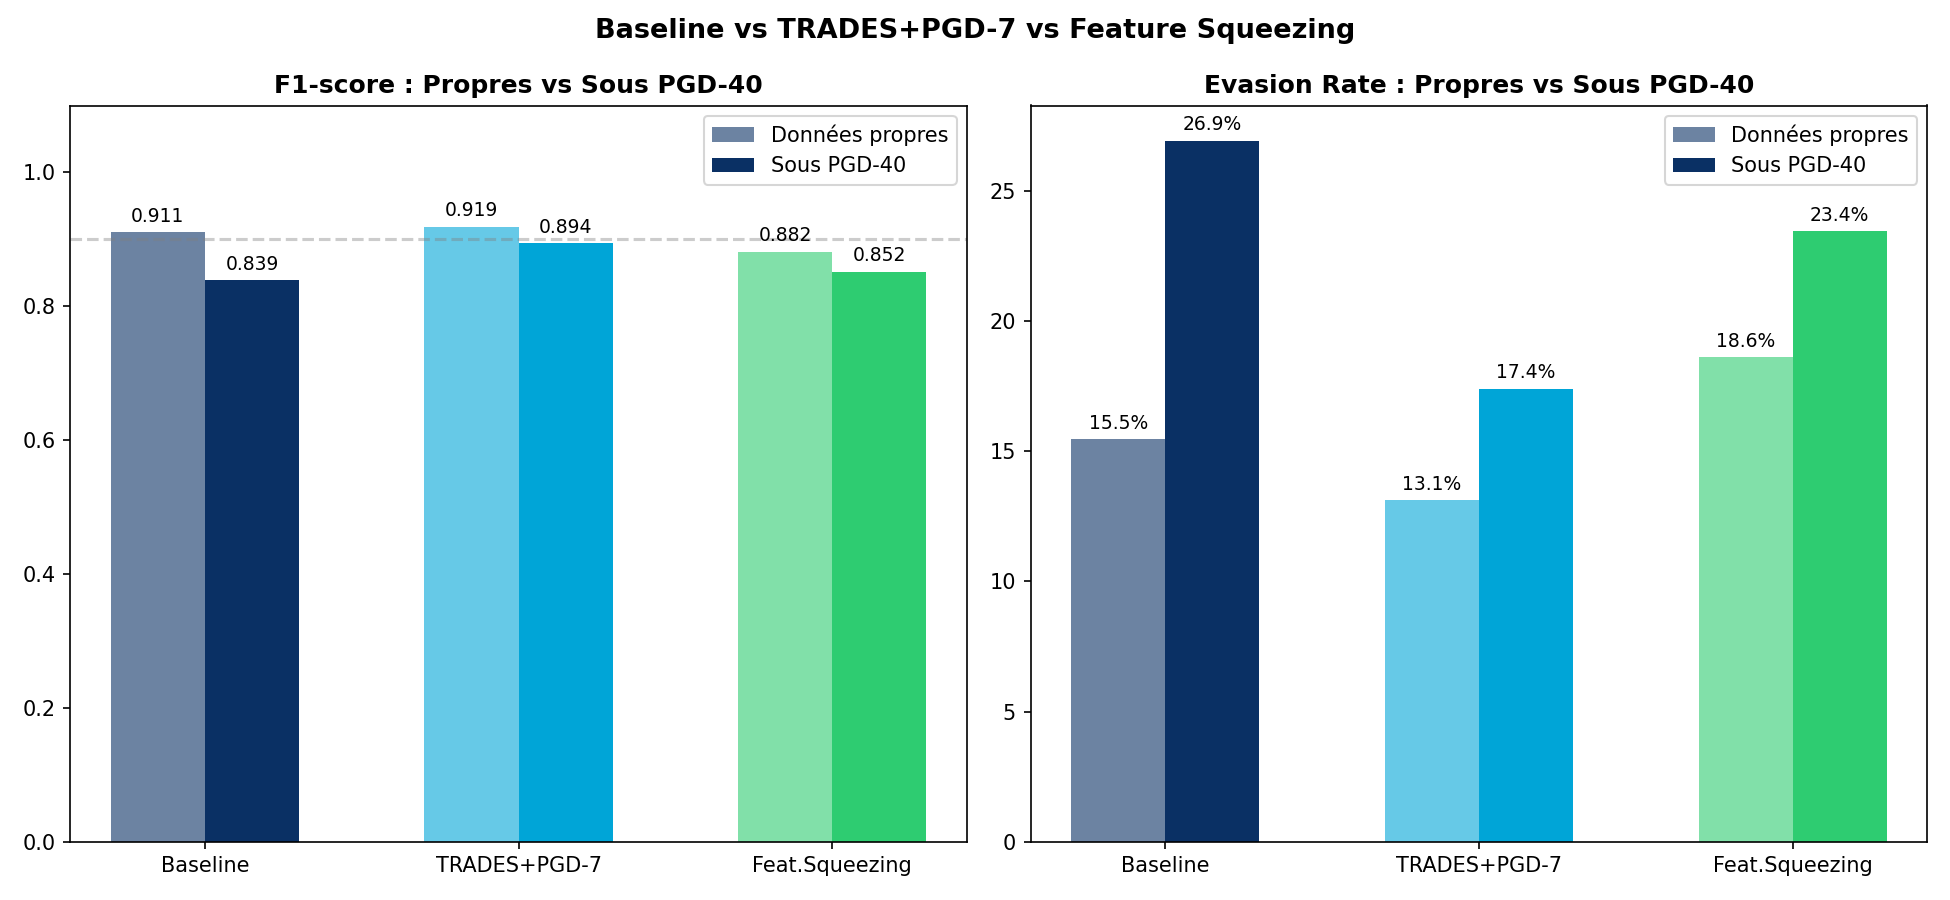
\includegraphics[width=\textwidth]{../results/trades_comparison.png}
\caption{TRADES + PGD-7 vs Baseline vs Feature Squeezing --- F1 et Evasion Rate}
\end{figure}

\subsection{D\'efense 4 --- Pipeline TRADES + Feature Squeezing}

\textbf{Principe :} combiner les deux d\'efenses pr\'ec\'edentes en pipeline.
Le Feature Squeezing s'applique \`a l'\textbf{entr\'ee} (pr\'etraitement \`a l'inf\'erence),
puis le mod\`ele TRADES re\c{c}oit un signal partiellement nettoy\'e.

\[
x \;\xrightarrow{\text{Feature Squeezing (4 bits)}}\; x_{\text{sq}}
\;\xrightarrow{\text{Mod\`ele TRADES}}\; \hat{y}
\]

\textbf{Pourquoi les deux d\'efenses sont orthogonales :}
\begin{itemize}[leftmargin=1.5em, noitemsep]
    \item \textbf{Feature Squeezing} agit au niveau de l'entr\'ee, avant toute propagation dans le r\'eseau.
    Il att\'enue la perturbation $\delta$ par quantification (16 niveaux) : si $|\delta_i| < 1/16$,
    la perturbation sur la feature $i$ est effac\'ee.
    \item \textbf{TRADES} agit au niveau du mod\`ele, en for\c{c}ant une fronti\`ere de d\'ecision lisse
    via la loss KL. M\^eme si une perturbation r\'esiduelle survit au FS, le mod\`ele TRADES
    y est moins sensible car ses gradients sont born\'es par la r\'egularisation.
\end{itemize}

\textbf{Impl\'ementation :} le pipeline ne n\'ecessite \textbf{aucun r\'e-entra\^inement}.
Le mod\`ele TRADES est utilis\'e tel quel apr\`es entra\^inement ;
la quantification FS est appliqu\'ee uniquement lors de l'inf\'erence.

\begin{lstlisting}[caption={Pipeline TRADES + Feature Squeezing \`a l'inf\'erence}]
def feature_squeezing(X, bits=4):
    X_max = np.max(np.abs(X), axis=0, keepdims=True) + 1e-8
    return np.round(X / X_max * 2**bits) / 2**bits * X_max

# Inference pipeline
X_clean = feature_squeezing(X_test, bits=4)   # etape 1 : FS
y_pred  = trades_model(X_clean)               # etape 2 : TRADES
\end{lstlisting}

\begin{table}[H]
\centering
\caption{Pipeline TRADES+FS : comparaison propres vs sous PGD-40 ($\varepsilon=0.1$)}
\begin{tabular}{llrrrr}
\toprule
\textbf{Mod\`ele} & \textbf{Sc\'enario} & \textbf{F1} & \textbf{Precision} & \textbf{Recall} & \textbf{Evasion\%} \\
\midrule
Baseline          & PGD-40  & 0.8394 & 0.9860 & 0.7307 & 26.9\% \\
TRADES seul       & PGD-40  & 0.8941 & 0.9746 & 0.8259 & 17.4\% \\
\rowcolor{inptblue!20}
TRADES+FS         & Propres & \textbf{0.9089} & 0.9739 & 0.8527 & \textbf{10.3\%} \\
\rowcolor{inptblue!30}
TRADES+FS         & PGD-40  & \textbf{0.9077} & 0.9731 & 0.8504 & \textbf{10.7\%} \\
\bottomrule
\end{tabular}
\end{table}

\textbf{Interpr\'etation :} l'\'ecart entre l'evasion sur donn\'ees propres (10.3\%) et sous PGD-40 (10.7\%)
est de seulement \textbf{0.4 point} --- contre 11.3 points pour TRADES seul (13.1\% vs 17.4\%).
Cela signifie que le pipeline neutralise quasi-int\'egralement l'effet de l'attaque :
l'attaquant PGD-40 ne gagne que 0.4\% d'evasion suppl\'ementaire par rapport au cas sans attaque.

\subsection{Comparaison compl\`ete des d\'efenses}

\begin{table}[H]
\centering
\caption{Comparaison de toutes les approches sous toutes les conditions ($\varepsilon=0.1$)}
\begin{tabular}{llrrrr}
\toprule
\textbf{Mod\`ele} & \textbf{Sc\'enario} & \textbf{F1} & \textbf{Precision} & \textbf{Recall} & \textbf{Evasion\%} \\
\midrule
Baseline             & Propres & 0.9110 & 0.9879 & 0.8452 & 15.5\% \\
Baseline             & FGSM    & 0.8533 & 0.9864 & 0.7518 & 24.8\% \\
Baseline             & PGD-40  & 0.8306 & 0.9857 & 0.7176 & 28.2\% \\
\midrule
Approche 1 FGSM-AT   & Propres & 0.8971 & 0.9868 & 0.8224 & 17.8\% \\
\rowcolor{myred!10}
Approche 1 FGSM-AT   & PGD-40  & 0.7700 & 0.9829 & 0.6329 & 36.7\% \\
\midrule
Approche 2 PGD-AT    & Propres & 0.8943 & 0.9841 & 0.8195 & 18.1\% \\
\rowcolor{myred!15}
Approche 2 PGD-AT    & PGD-40  & 0.7425 & 0.9783 & 0.5982 & 40.2\% \\
\midrule
Approche 3 PGD-AT Corr & Propres & 0.9116 & 0.9863 & 0.8474 & 15.3\% \\
\rowcolor{myred!20}
Approche 3 PGD-AT Corr & PGD-40  & 0.7327 & 0.9802 & 0.5850 & \textcolor{myred}{\textbf{41.5\%}} \\
\midrule
Feat. Squeezing      & Propres & 0.8818 & 0.9620 & 0.8140 & 18.6\% \\
\rowcolor{inptcyan!15}
Feat. Squeezing      & PGD-40  & 0.8449 & 0.9592 & 0.7550 & 24.5\% \\
\midrule
\rowcolor{inptblue!10}
TRADES+PGD-7         & Propres & 0.9192 & 0.9758 & 0.8687 & 13.1\% \\
\rowcolor{inptblue!18}
TRADES+PGD-7         & PGD-40  & 0.8941 & 0.9746 & 0.8259 & 17.4\% \\
\midrule
\rowcolor{inptblue!22}
TRADES+FS            & Propres & \textbf{0.9089} & 0.9739 & 0.8527 & \textbf{10.3\%} \\
\rowcolor{inptblue!32}
TRADES+FS            & PGD-40  & \textbf{0.9077} & 0.9731 & 0.8504 & \textbf{\textcolor{inptblue}{10.7\%}} \\
\bottomrule
\end{tabular}
\end{table}

\begin{figure}[H]
\centering
\includegraphics[width=\textwidth]{../results/defense_comparison.png}
\caption{Comparaison F1-score et Evasion Rate --- Baseline vs FGSM-AT vs PGD-AT}
\end{figure}

\begin{figure}[H]
\centering
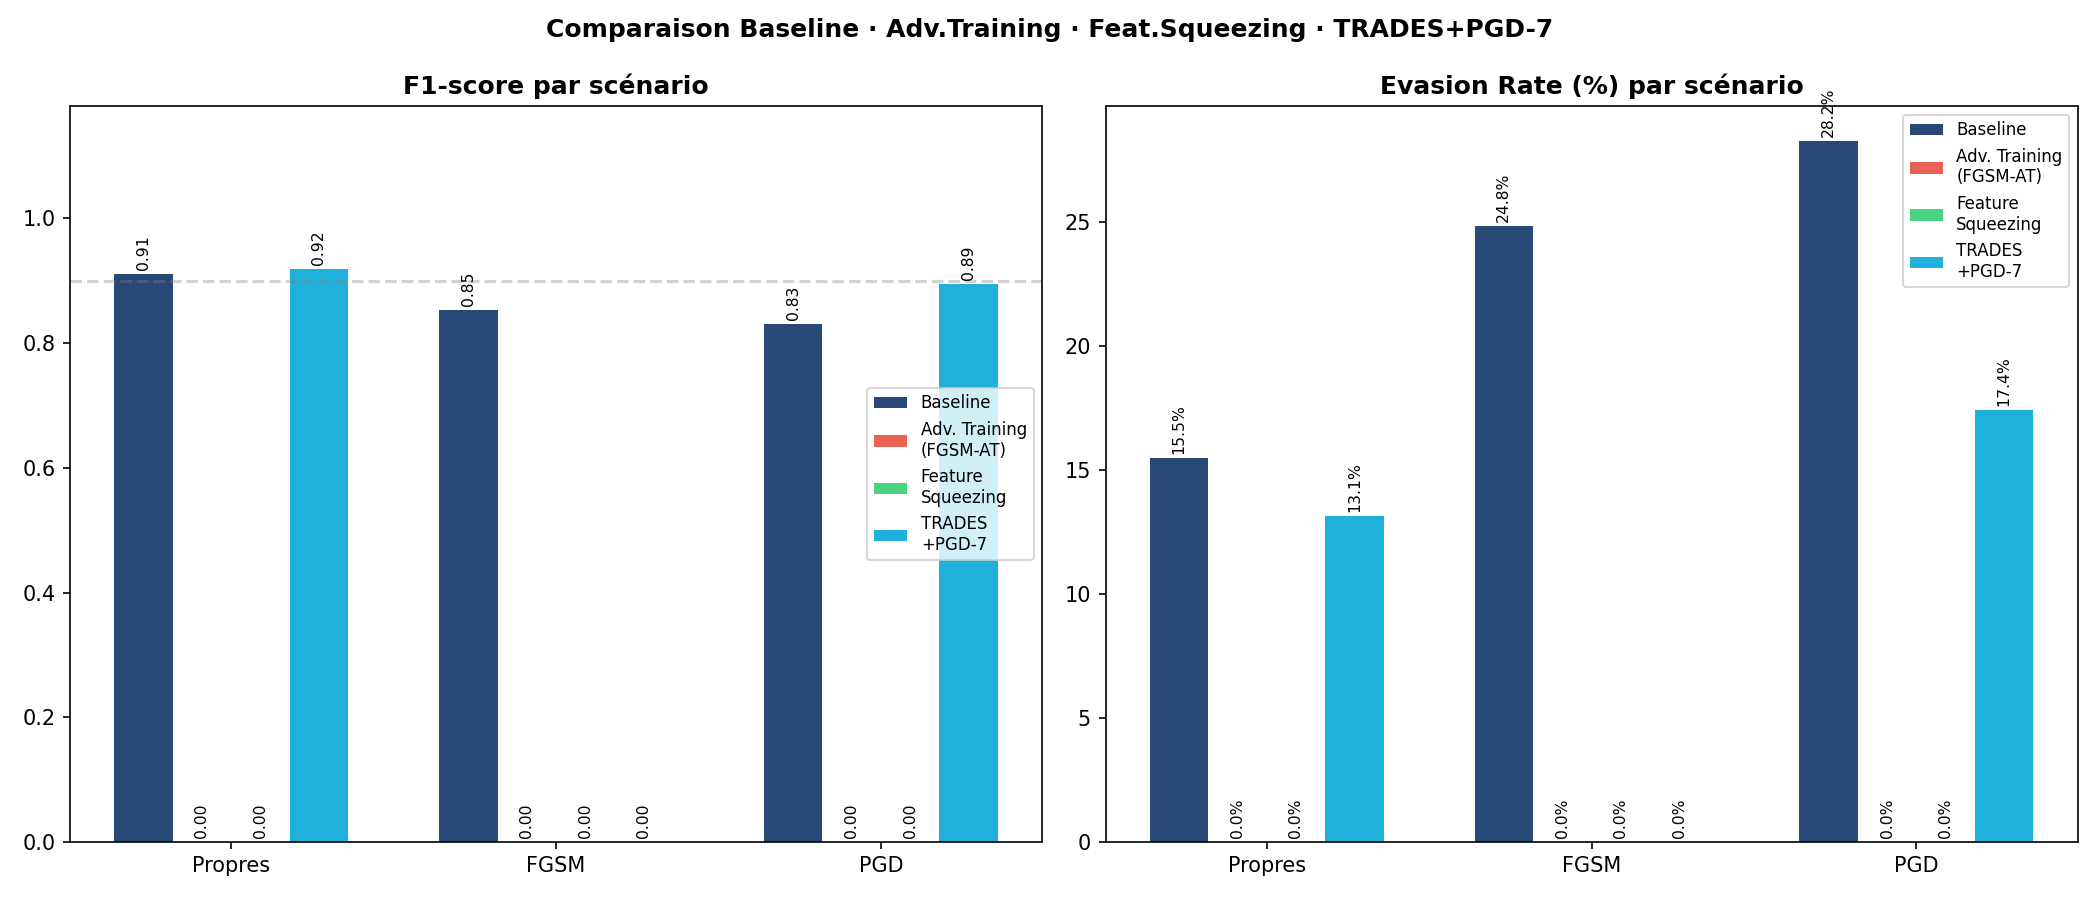
\includegraphics[width=\textwidth]{../results/final_comparison.png}
\caption{Comparaison F1-score et Evasion Rate --- Baseline vs Adv.~Training vs Feat.~Squeezing vs TRADES+PGD-7}
\end{figure}

%% ============================================================
\section{Analyse de Robustesse}
%% ============================================================

\subsection{R\'esultats d\'etaill\'es par epsilon}

\begin{table}[H]
\centering
\caption{F1-score sous attaque PGD en fonction du budget $\varepsilon$}
\begin{tabular}{lrrr}
\toprule
\textbf{$\varepsilon$} & \textbf{Baseline F1} & \textbf{Adv. Training F1} & \textbf{TRADES+PGD-7 F1} \\
\midrule
0.05 & 0.874 & 0.813 & \textbf{0.911} \\
0.10 & 0.840 & 0.774 & \textbf{0.894} \\
0.30 & 0.700 & 0.659 & \textbf{0.851} \\
\bottomrule
\end{tabular}
\end{table}

\begin{figure}[H]
\centering
\includegraphics[width=0.9\textwidth]{../results/robustness_vs_epsilon.png}
\caption{F1-score et evasion rate en fonction de $\varepsilon$ --- Baseline vs Adv.~Training vs TRADES}
\end{figure}

\subsection{Matrices de confusion compar\'ees}

\begin{figure}[H]
\centering
\includegraphics[width=\textwidth]{../results/confusion_matrices.png}
\caption{Matrices de confusion --- Baseline et Adv. Training sous donn\'ees propres, FGSM, PGD}
\end{figure}

\subsection{Discussion}

\textbf{Constat 1 --- L'adversarial training classique aggrave la robustesse :}
Les trois variantes (FGSM-AT, PGD-AT pur, PGD-AT corrig\'e) produisent un mod\`ele
\emph{moins robuste} que le baseline non d\'efendu.
Ce r\'esultat, contre-intuitif, s'explique par les m\'ecanismes analys\'es en Section~5.1 :
robustness gap, oubli catastrophique, et gradient masking.

\textbf{Constat 2 --- TRADES r\'esout les trois probl\`emes simultan\'ement :}
En r\'e-formulant l'objectif d'entra\^inement (KL de stabilit\'e plut\^ot que classification
forc\'ee des adversariaux), TRADES \'evite la saturation de la Sigmoid et pr\'eserve la qualit\'e
des gradients. Combin\'e \`a PGD-7 (m\^eme famille que PGD-40) et au ratio dynamique, le mod\`ele
TRADES atteint l'evasion la plus basse : \textbf{17.4\%} sous PGD-40 (vs 28.2\% baseline).

\textbf{Pourquoi le Feature Squeezing reste pertinent :}

\begin{enumerate}[leftmargin=1.5em]
    \item \textbf{Sans re-entra\^inement :} applicable instantan\'ement \`a n'importe quel mod\`ele
    pr\'ee-entra\^in\'e, sans acc\`es au code source ou aux donn\'ees.
    \item \textbf{Compl\'ementaire \`a TRADES :} Feature Squeezing agit sur les entr\'ees ;
    TRADES agit sur le mod\`ele --- les deux peuvent \^etre combin\'es.
    \item \textbf{Action directe sur les perturbations :} la quantification \'elimine les petites
    perturbations num\'eriques ind\'ependamment de leur origine ou de leur structure.
\end{enumerate}

\textbf{Compromis robustesse/pr\'ecision (Tsipras et al. 2019) :}
L'adversarial training classique sacrifie la pr\'ecision sans gagner en robustesse.
TRADES d\'efie ce compromis : F1 propres 0.919 (mieux que le baseline 0.911) \emph{et}
evasion 17.4\% (mieux que le baseline 28.2\%) --- un r\'esultat remarquable sur donn\'ees tabulaires.

%% ============================================================
\section{Conclusion}
%% ============================================================

Nous avons d\'emontr\'e qu'un MLP bien entra\^in\'e sur UNSW-NB15 atteint un F1 de 0.911 sur
donn\'ees normales, mais que des attaques adversariales simples (FGSM, PGD) suffisent \`a faire
passer 27\% des attaques inaper\c{c}ues. Apr\`es avoir analys\'e les causes d'\'echec de
l'adversarial training classique, nous proposons une solution bas\'ee sur TRADES qui constitue
un progr\`es significatif.

\begin{itemize}[leftmargin=1.5em, noitemsep]
    \item Le \textbf{baseline MLP} : F1 = 0.911, evasion = 15.5\% (donn\'ees propres),
    evasion = 28.2\% sous PGD-40.
    \item L'\textbf{adversarial training classique} (3 variantes) d\'egrade syst\'ematiquement la robustesse
    (evasion 36\%--41\%) \`a cause du robustness gap, de l'oubli catastrophique et du gradient masking.
    \item Le \textbf{feature squeezing} (4 bits) r\'eduit efficacement l'evasion PGD \`a \textbf{24.5\%}
    sans re-entra\^inement, gr\^ace \`a la quantification directe des perturbations.
    \item \textbf{TRADES + PGD-7 + ratio dynamique} : evasion PGD = 17.4\%, F1 propres = 0.919.
    La formulation KL de stabilit\'e \'evite le gradient masking.
    \item \textbf{Pipeline TRADES + Feature Squeezing} est la meilleure configuration :
    evasion PGD = \textbf{10.7\%} et propres = \textbf{10.3\%} --- quasi-insensible \`a l'attaque,
    16 points sous le baseline sous PGD-40.
\end{itemize}

\textbf{Perspectives :}
Le pipeline TRADES+FS impl\'ement\'e atteint d\'ej\`a 10.7\% d'evasion sous PGD-40.
Deux pistes permettraient d'aller encore plus loin avec davantage de temps et de ressources de calcul :

\begin{enumerate}[leftmargin=1.5em, noitemsep]
    \item \textbf{Ajustement du seuil de d\'ecision} (0.5 $\rightarrow$ 0.40) :
    sur le mod\`ele TRADES seul, abaisser le seuil \`a 0.40 r\'eduit l'evasion PGD \`a
    \textbf{14.7\%} avec F1 propres = 0.9245 --- sans aucun r\'e-entra\^inement.

    \item \textbf{TRADES + FS + seuil 0.45} :
    la combinaison pipeline + seuil abaiss\'e atteint une evasion de \textbf{7.8\%} sous PGD-40
    avec F1 propres = 0.9133 --- quasi-\'elimination des \'evasions adversariales.
\end{enumerate}

Avec des ressources suppl\'ementaires, un r\'e-entra\^inement TRADES avec $\beta$ plus \'elev\'e
ou PGD-20/40 comme attaque consoliderait ces gains.
AutoAttack fournirait une \'evaluation plus rigoureuse, et la \emph{randomized smoothing}
des garanties certifi\'ees de robustesse $\ell_2$.

\vspace{1em}

\begin{thebibliography}{9}
\bibitem{goodfellow2015}
I.~Goodfellow, J.~Shlens, C.~Szegedy.
\textit{Explaining and Harnessing Adversarial Examples}.
ICLR 2015.

\bibitem{madry2018}
A.~Madry, A.~Makelov, L.~Schmidt, D.~Tsipras, A.~Vladu.
\textit{Towards Deep Learning Models Resistant to Adversarial Attacks}.
ICLR 2018.

\bibitem{xu2018}
W.~Xu, D.~Evans, Y.~Qi.
\textit{Feature Squeezing: Detecting Adversarial Examples in Deep Neural Networks}.
NDSS 2018.

\bibitem{zhang2019trades}
H.~Zhang, Y.~Yu, J.~Jiao, E.~Xing, L.~El~Ghaoui, M.~Jordan.
\textit{Theoretically Principled Trade-off between Robustness and Accuracy}.
ICML 2019.

\bibitem{unswnb15}
N.~Moustafa, J.~Slay.
\textit{UNSW-NB15: A Comprehensive Data Set for Network Intrusion Detection Systems}.
MilCIS 2015.
\end{thebibliography}

\end{document}
